

\chapter{Focus structures in ZAI}\label{focuschapter} 

In this chapter, I move away from the discussion of the specific forms of ZAI nominals and the ways that these signal more or less accessible referents and turn towards an analysis of the information structure categories of topic and focus. Topic and focus relations involve the relations not between discourse referents and accessibility but between discourse referents and propositions. That is, in similar sentences uttered in different contexts, the cognitive status of two referents may be the same, but the function -- i.e. topic or focus -- may be different; as such, cognitive status is only a precondition for the expression of these functions \citep{lambrecht1994}. The analysis below focuses on pragmatic phenomena that have particular correlates in clause or sentence structure. As we will see from the analysis that follows, the flexible nature of constituent order in ZAI is an important resource for ZAI speakers in organizing information structure.

This chapter aims to show that ZAI is a verb-initial language that displays flexible syntax whose linear order is strongly motivated by the pragmatic function of the utterance. In particular, linear order is determined in large part by decisions made by the speaker with respect to what the proposition is about, what is contextually dependent, what is pragmatically presupposed, and what is asserted. The following chapter, \sectref{topicchapter}, explores related phenomena from the perspective of ZAI topic relations. 

In what follows, I investigate the organization of focus structure in ZAI again with an emphasis on the ways that the various typological characteristics of the language -- phonological, morphological, and syntactic -- interact with each other. The ZAI data supports the hypothesis that ZAI speakers mark focus relations primarily through the manipulation of constituent order and/or through morphological marking (for other Zapotec languages, see \citealt{broadwell1999b,lee2000}) rather than through prosodic means. There does not seem to be any evidence for any pitch accents directly associated with focal material, although elements may display various prosodic properties-- duration, pitch register, and pitch range-- that may be related to the position within a given intonation unit in which they appear.

The chapter begins with a discussion of focus structure in ZAI and an analysis of the conceptualization of \citet{lambrecht1994} as it applies it to the ZAI data. In the section that follows, I introduce the typology of focus structure proposed by \citet{vanvalin1999} and examine the place of ZAI within that typology. I then present and discuss a conversational strategy by ZAI speakers involving the parallel, chiastic use of predicate focus and argument focus to accomplish specific conversational goals. 


\section{Focus structure}

The term \textit{focus structure} \citep{lambrecht1994} refers to the grammatical means by which a language indicates the scope of the assertion in an utterance and differentiates it from the presupposed or topical material.

The main contrast in focus structure is between broad focus and argument focus. Whereas in broad focus the focus domain extends over more than one constituent, in argument focus the focus domain extends only over one constituent. In broad focus constructions --which invariably involve verb-initial structures in ZAI-- the verb is part of the assertion. In narrow focus constructions, the verb is part of the presupposition. In ZAI,  narrow focus constructions tend strongly to not be verb-initial. The relevant generalization is the following: the verb will form part of the focus domain unless the construction is an argument focus construction, in which case it forms part of the presupposition.  

There are two types of broad focus, predicate focus and sentence focus. I address these in turn.


\subsection{Predicate focus}\label{pfsection}

Predicate focus is traditionally referred to as a topic-comment construction, as in \sectref{topiccommentsection}, where the subject is the topic and the predicate is a comment on that topic. This is the unmarked focus type. The following examples from \citet{lambrecht1994} illustrate this focus construction type in four different languages, English, Italian, French, and Japanese. The sentences represent a prototypical response in each respective language to the question ``How's your car?'' which establishes ``my car'' as the topic (boldface indicates focal stress). 


\ea\label{PF}Q: \textit{How's your car?}
\begin{table} 
\begin{tabular}{l l l l}
 & a. & \textit{My car/it broke \textbf{down}}. & \textit{English} \\
 & b. & \textit{(La mia macchina) si \`{e} \textbf{rotta}}. & \textit{Italian} \\
 & c. & \textit{(Ma voiture) elle est en \textbf{panne}}. & \textit{French} \\
  & d. & \textit{(Kuruma wa) \textbf{koshoo}shita}. & \textit{Japanese} \\
\end{tabular}
\end{table}
\z

In each case, the predicate is a comment or assertion about the subject-topic ``my car''. In English and Italian, the subject NP is the topic. In French, it is a detached NP, and, in Japanese, it is a \textit{wa}-marked NP. In each of these languages the order of constituents is S-V and there is focal stress on the verb. 

The realization of predicate focus is substantially different in ZAI, where predicate focus constructions are verb-initial: 
\ea\label{predfoc1}
\glll guxhii\~{n}e xcoch\'{e}'  \\
gu-xhii\~{n}e' x=coche=e'\textsuperscript{H}  \\
\textsc{compl}-break.down \textsc{poss}-car=\textsc{1sg}  \\
\glt `My car broke down'
\z
Although the subject-topic may be a full NP, as above, a subject pronominal clitic is more common:
\ea\label{predfoc2}
\glll guxhii\~{n}en\v{i} \\
gu-xhii\~{n}e'=ni\textsuperscript{LH}  \\
\textsc{compl}-break.down=\textsc{3.inan} \\
\glt `It broke down'
\z
The predicate thus occupies the clause-initial position in ZAI followed by the subject-topic, which can be realized as an enclitic or as a full NP.\footnote{Predicate focus with a transitive verb and two full NP arguments would require the topical subject NP to appear before the verb. However, because topical subjects are very rarely coded using full NPs, this word order occurs in my corpus only in elicitation contexts.}

Below is a second example of a prototypical predicate focus construction in ZAI:

\ea\label{predfocus}
{Q: What did the boy do?} \\
\glll bidxaagabe t\'{i} dxaapahuiini' \\
bi-dxaaga=be\textsuperscript{LH} ti dxaapa-huiini' \\
\textsc{compl}-encounter=\textsc{3.hum} one girl-\textsc{dim} \\
\glt `He encountered a girl' 
\z
This is a transitive clause where the subject-topic, `the boy', appears as an enclitic on the verb and the predicate, `encountered a girl' is the comment or assertion about the subject-topic. Again, this is a verb-initial construction.

The verb and the object are in the focus domain in this case, but neither receive focal stress in the form of a pitch accent. There is a gradual downdrift in pitch from the beginning of the clause to the end, but no specific pitch accent occurs on either the verb or the object. The one H tone in the clause surfaces on \textit{ti} as a result of the floating tone from the third person enclitic \textit{=be}. This can be observed in the pitch track of this utterance shown below:

\vspace{3mm}

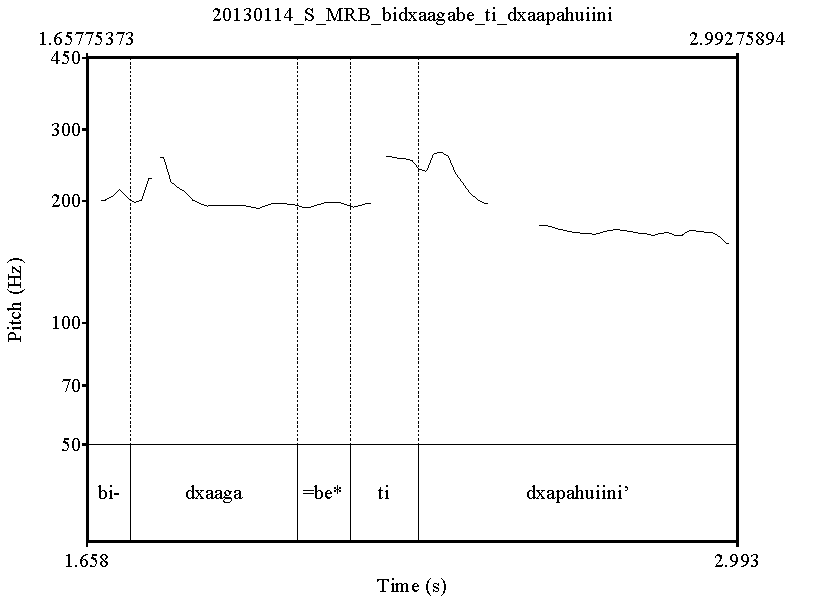
\includegraphics[height=.4\textheight]{dxaapahuiini}

In general, elements that appear at the beginning of the intonation unit are pronounced with longer duration, a higher pitch register and wider pitch range, i.e. properties associated with beginnings and endings of intonation units. In this case, it is the verbal constituent that occurs in the prosodically more prominent position, the beginning of the intonation unit. The object NP constituent occurs in the next most prosodically prominent position, the end of the intonation unit.

Consider, now, the following example, taken from conversation:

\ea\label{guetijugo} (M 18 March 2012, 08:47.0-08:52.0)
\begin{itemize}
\item [01]
\glll biban\'{e} l\'{a}, \\
bi-bani=a'\textsuperscript{H} la\textsuperscript{H} \\
\textsc{compl}-wake.up=\textsc{1sg} \textsc{la} \\
\glt `I woke up,' 


\item [02]
\glll guz\'{e} xa \\
gu-zi=a'\textsuperscript{H} xa \\
\textsc{compl}-shower=\textsc{1sg} \textsc{intj} \\
\glt `I showered,' 


\item [03]
\glll g\"{u}\'{e} ti j\v{u}go de nar\v{a}njasi x\'{a} \\
g\"{u}-e-a'\textsuperscript{H} ti ju\textsuperscript{LH}go de nara\textsuperscript{LH}nja-si\textsuperscript{LH} xa \\
\textsc{compl}-drink=\textsc{1sg} one juice of orange-only \textsc{intj} \\
\glt `I drank an orange juice only.'

\end{itemize}
\z
Here, the speaker remembers and tells about the sequential events during a morning routine. Each of the three lines is a predicate focus construction. Each clause is verb-initial, with the narrator as the subject-topic and each predicate advancing the events in the narrative. 

As seen below, in this case as well, there is no pitch accent associated with any of the constituents of the sentence. 

\vspace{3mm}

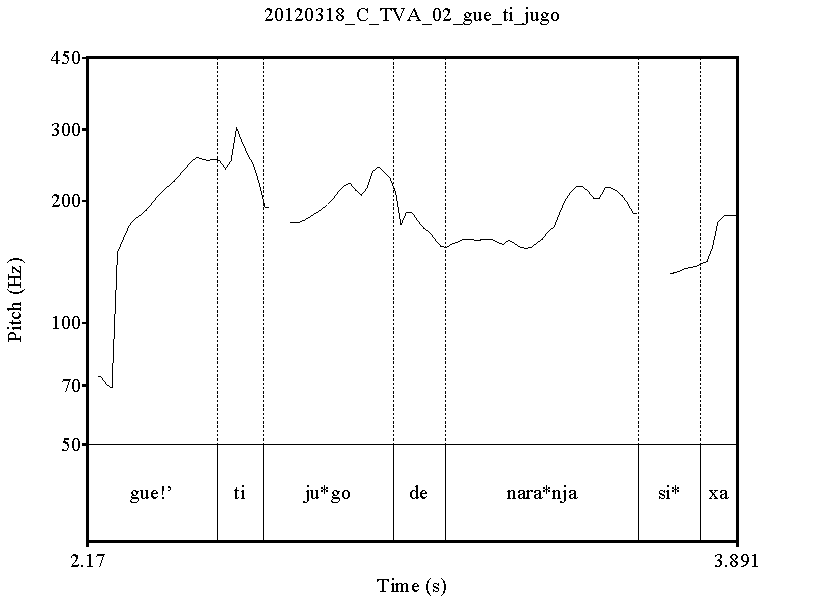
\includegraphics[height=.4\textheight]{guetijugo}

In the last line, line 3, The H and LH tones that surface can be directly attributed to the underlying tones. The verb \textit{g\"{u}e} carries a H tone from the first person enclitic. The NPs \textit{jugo} and  \textit{nar\v{a}nja} both carry an LH tone on the stressed syllable, as is characteristic of many Spanish loanwords. Finally, the particle \textit{-si} attached to the object NP contains a floating H tone that surfaces on the final particle \textit{xa}. 

The principal characteristic of predicate focus constructions in ZAI, therefore, is that they involve a verb-initial main clause. Again, the verb is part of the focus domain and does not receive focal stress in the form of a pitch accent. Additionally, there is a gradual downdrift in pitch from the beginning of the clause to the end, but no specific pitch accent occurs on the object either. Below, we will compare predicate focus constructions to argument focus constructions in which a different constituent may occupy the pre-verbal position. First, I discuss sentence focus constructions, which are also verb-initial.



\subsection{Sentence focus}\label{sfsection}

I turn now to sentence focus, discussed previously in \sectref{presentationalsection} as presentational or event-reporting constructions. In these, there is no topical subject and the focus domain is the entire sentence (again, examples are from \citet{lambrecht1994}). 


\ea\label{SF}
{Q: What happened?} \\
\begin{table} 
\begin{tabular}{l l l l}
 & a. & \textit{My \textbf{car} broke down}. & \textit{English} \\
 & b. & \textit{Mi si \`{e} rotta la \textbf{macchina}}. & \textit{Italian}  \\
  & & Lit. `Broke down to me the car'  \\
 & c. & \textit{J'ai ma \textbf{voiture} qui est en panne}. & \textit{French}  \\
  & & Lit. `I have my car which broke down' \\
   & d. & \textit{\textbf{Kuruma} ga \textbf{koshoo}shita}. & \textit{Japanese}  \\
\end{tabular}
\end{table}
\z

Unlike the examples of predicate focus listed in (\ref{PF}), each of the sentences in (\ref{SF}) lack a presupposed topic and, instead, the entire sentence is asserted. English uses the same syntactic construction as in (\ref{PF}), however, in this case the subject NP receives focal stress. In Italian, the focal stress still falls on the final constituent of the sentence, but the syntactic construction is altered so that the focused subject NP appears sentence-finally. In French, both the focal stress and the syntactic construction differ from (\ref{PF}) and a part of the information is now communicated via a relative clause.  In Japanese, both the subject and the verb receive focal stress and the subject is marked using the morpheme \textit{ga} rather than \textit{wa}.

In ZAI, the construction is formally identical to the predicate focus construction in (\ref{predfoc1}), except in this case there is no option to represent the subject as an enclitic. It must appear as a lexical NP:
\ea 
\glll guxhii\~{n}e xcoch\'{e}' \\
gu-xhii\~{n}e' x=coche=e'\textsuperscript{H} \\
\textsc{compl}-break.down \textsc{poss}-car=\textsc{1sg} \\
\glt `My car broke down'
\z

As we will see in the discussion of event-reporting constructions in \sectref{presentationalsection}, the most common use of sentence focus constructions is presentational constructions, to introduce new participants to a discourse. Consider the following example taken from a Pear Story narrative:

\ea
\glll bihuinni ti r\'{i}gola  \\
bi-huinni ti ri\textsuperscript{H}gola \\
\textsc{compl}-appear one man \\
\glt `A man appeared' 
\z
In a typical use such as this, the narrator uses a sentence focus construction to introduce a participant into the discourse. As with predicate focus, this is also a verb-initial construction which places the verb in the most prominent prosodic position. The intransitive subject is introduced as an indefinite noun and occupies the position at the end of the intonation unit. There is no topical subject and the focus domain is the entire sentence. Here, again, there is no special pitch accent associated with this construction.  


\subsection{Argument focus}\label{afsection}

While predicate focus and sentence focus are both types of broad focus, argument focus involves narrow focus. In argument focus, referred to as an identificational construction in \sectref{identificationalsection}, the focus domain is a single constituent, which may be an object, subject, adjunct, or even a verb (examples are from \citet{lambrecht1994}).


\ea\label{AF}
{Q: I heard your motorcycle broke down.} \\
\begin{table} 
\begin{tabular}{l l l l}
 & a. & \textit{My \textbf{car} broke down}. & \textit{English} \\
 & a'. & \textit{It's my \textbf{car} that broke down}. \\
 & b. & \textit{Si \`{e} rotta la mia \textbf{macchina}}. & \textit{Italian} \\
  & & Lit. `Broke down my car' \\
   & b'. & \textit{\`{E} la mia \textbf{macchina} che si \`{e} rotta}. \\
     & & Lit. `It's my car that broke down' \\
 & c. & \textit{C'est ma \textbf{voiture} qui est en panne}. & \textit{French} \\
  & & Lit. `It's my car that broke down'  \\
   & d. & \textit{\textbf{Kuruma} ga koshooshita}.  & \textit{Japanese} \\
\end{tabular}
\end{table}
\z

In these sentences, the focus domain is restricted to the NP \textit{car}. The presupposition is that `something broke down' and the assertion is that it was the speaker's car and not something else that broke down. English again uses the same syntactic S-V-O construction and, as in (\ref{SF}), the subject NP again receives focal stress. In Italian, the syntactic construction is altered in such a way that the focal stress again falls on the final constituent of the sentence. In French, both the focal stress and the syntactic construction again differ from (\ref{PF}) and (\ref{SF}), with a part of the information again being communicated via a relative clause. In Japanese, the subject is marked using the morpheme \textit{ga} (as in (\ref{SF}d)), and only the subject NP receives focal stress.

In argument focus it is possible for the focused NP to occur post-verbally in ZAI, but this is much less common and the preferred order is the following, where the focused NP constituent appears pre-verbally in clause-initial position: 
\ea 
\glll xcoch\'{e}' guxhii\~{n}e' \\
x=coche=e'\textsuperscript{H} gu-xhii\~{n}e'  \\
\textsc{poss}-car=\textsc{1sg} \textsc{compl}-break.down  \\
\glt `My CAR broke down'
\z

Below is an example taken from conversation:

\ea(T and M, 18 March 2012, 16:03.0-16:06.0)
\begin{itemize}
\item[01 T:]
\glll tu l\'{a} bini gan\'{a}r, este, prim\'{e}r lug\'{a}r? \\
tu\textsuperscript{LH} la\textsuperscript{LH} b-ini ganar\textsuperscript{H} este primer\textsuperscript{H} lugar\textsuperscript{H} \\
who name \textsc{compl}-do win \textsc{intj} first place  \\
\glt `Who won, um, first place?'


\item[02 M:]
\glll ti milit\'{a}r bini gan\'{a}r dxiqu\v{e} \\
ti militar\textsuperscript{H} bi-ini ganar\textsuperscript{H} dxique\textsuperscript{LH} \\
one soldier \textsc{compl}-do win then \\
\glt `A SOLDIER won then' 


\end{itemize}
\z
Here, the question in line 1 by speaker V introduces the presupposition 'x won first place'. Speaker M responds in line 2 with the assertion `x is a soldier' and uses a construction in which the subject appears in pre-verbal position followed by the verb which forms part of the presupposition. The most prominent prosodic position is occupied in this case by the subject NP.

Consider the following example, also of an argument focus construction. Here, the speaker's own statement in line 1 sets up a presupposition which is followed in line 2 by an argument focus construction.  

\ea\label{jugoquesigue}(M, 18 March 2012, 10:20.5-10:23.5)
\begin{itemize}
\item [01]
\glll nin qu\'{i} \~{n}ahuadi\'{a} de endar\'{e} gast\'{i}' \\
nin qui \~{n}-ahua-di=a'\textsuperscript{H} de guendaro=a'\textsuperscript{H} gasti'\textsuperscript{H}  \\
not.even \textsc{neg} \textsc{irr}-eat/drink-\textsc{neg}=\textsc{1sg} of food=\textsc{1sg} nothing \\
\glt `I didn't even eat/drink any of my food'


\item [02]
\glll j\v{u}go ques\'{i} gu\'{e}' \\
ju\textsuperscript{LH}go que\textsuperscript{LH}-si\textsuperscript{LH} gu-e=a'\textsuperscript{H} \\
juice \textsc{dem}-only \textsc{compl}-eat/drink=\textsc{1sg} \\
\glt `I drank ONLY THE JUICE.'  

\end{itemize}
\z
Note first that the verb `to eat/drink' is the same verb in line 1 as in line 2, the phonological form of the verb is conditioned by the TAM prefix. In line 1, the speaker sets up the presupposition 'I ate/drank x'. He continues in line 2 with the assertion 'x is only the juice.'  

It is not the verb but an NP constituent that is in the prosodically prominent position at the beginning of the intonation unit. As above, however, there is no particular pitch accent associated with any particular part of the utterance:

\vspace{3mm}

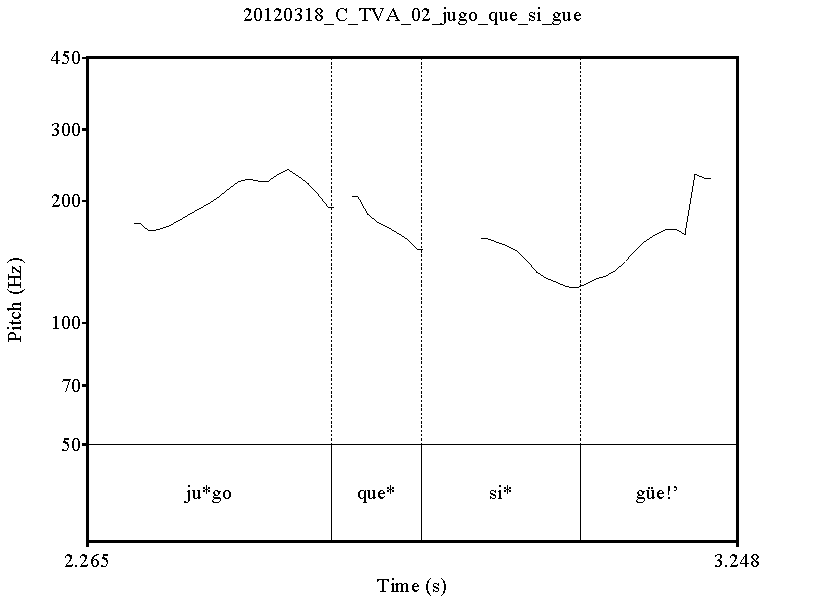
\includegraphics[height=.4\textheight]{jugoquesigue}

We can compare this construction to the predicate focus construction, `\textit{gue ti jugo de naranjasi xa}' in (\ref{guetijugo}) uttered by the same speaker. The constructions carry almost identical propositional content, except that in (\ref{guetijugo}) the speaker uses an indefinite object NP and in (\ref{jugoquesigue}) uses a definite object NP. The two utterances differ also in the order of constituents, with the object NP occurring pre-verbally in the argument focus construction (\ref{guetijugo}) and post-verbally in the predicate focus construction (\ref{jugoquesigue}). I return to pairs of utterances such as these in \sectref{chiasmus}, where I discuss the patterned use of predicate focus followed by argument focus in conversation and explore the combined discourse function of the two constructions. 

First, it should be noted, however, that argument focus constructions do not have to be NP-initial. A construction such as the following, with a verb-initial structure, would also be acceptable in the same situation:

\ea
\glll gu\'{e} j\v{u}go ques\v{i}  \\
gu-e=a'\textsuperscript{H} ju\textsuperscript{LH}go que\textsuperscript{LH}-si\textsuperscript{LH}  \\
\textsc{compl}-eat/drink=\textsc{1sg} juice \textsc{dem}-only  \\
\glt `I drank ONLY THE JUICE.'  

\z
There is no formal marking that separates this construction from a predicate focus construction, leaving it formally ambiguous. However, an NP in pre-verbal position unambiguously signals the focal nature of the NP. In verb-initial constructions, focus may fall on the verb. Only contextual information allows the participants to understand that the presupposition and assertion in the verb-initial version remain the same as in the original construction of line 2 in (\ref{jugoquesigue}). Still, while a verb-initial structure can alternatively be used to communicate argument focus, the use of a pre-verbal constituent will always signal argument focus, unless the pre-verbal element is a subject NP and a resumptive pronominal clitic appears on the verb, as in the case of topicalization (see \sectref{topicalizationsection}). 

In the following section, I turn to a related argument focus construction involving the use of the particle \textsc{nga}.

\subsection{The use of \textsc{nga} in argument focus}\label{ngaargfoc}

The particle \textsc{nga} carries a H tone and is used in two types of constructions. One is in copulative constructions, such as in (\ref{cop}), where \textsc{nga}, according to \citet[94]{pickett1998}, ``emphasizes" the subject:

\ea\label{cop}
\glll laabe ng\'{a} m\'{a}istru \\
laa=be\textsuperscript{LH} nga\textsuperscript{H} mai\textsuperscript{H}stru \\
base=3\textsc{sg} \textsc{nga} teacher \\
\glt `HE is a teacher' \hfill \citep[94]{pickett1998}
\z
In this example, the independent pronoun functions as the subject of the clause, followed by \textsc{nga}, and then \textit{maistru} `teacher'. This construction contrasts with the alternative copulative construction involving a zero-copula:
\ea\label{copzero}
\glll m\'{a}istru laab\v{e} \\
mai\textsuperscript{H}stru laa=be\textsuperscript{LH} \\
teacher base=3\textsc{sg}  \\
\glt `He is a teacher' 
\z
These two constructions differ in that while (\ref{cop}) is a type of argument focus construction, (\ref{copzero}) is an example of predicate focus. 

The \textsc{nga} particle may be used in other constructions as well. It may be used to ``emphasize" a subject of a transitive clause, as in (\ref{emphsubj}):
\ea\label{emphsubj}
\glll naa ng\'{a} bi'n\'{e} n\v{i} \\
naa nga\textsuperscript{H} bi-i'ni=a' ni\textsuperscript{LH} \\
1\textsc{sg} \textsc{nga} \textsc{compl}-d=1\textsc{sg} 3\textsc{inan} \\
\glt `I am the one who did it' \hfill \citep[98]{pickett1998}
\z
In these cases, a co-referring dependent pronoun appears as an enclitic on the verb. In addition, it may  be used to ``emphasize" a direct object, as in (\ref{emphobj}).
\ea\label{emphobj} 
\glll Ju\'{a}n nga biiyalu neegue' \\
Juan\textsuperscript{H} nga\textsuperscript{H} bi-uuya=lu' neegue' \\
Juan \textsc{nga} \textsc{compl}-see=2\textsc{sg} yesterday \\
\glt `It was Juan who you saw yesterday' \hfill \citep[98]{pickett1998}

\z
The function of the \textsc{nga} particle to provide ``emphasis", as described by \citet{pickett1998}, can be understood in terms of \citet{lambrecht1994} as narrow or argument focus. Yet, it differs from argument focus constructions in which \textsc{nga} is not present. Example (\ref{emphobj}) is not identical to (\ref{emphobj2}), the corresponding argument focus construction without the particle \textsc{nga}:

\ea\label{emphobj2}
\glll Ju\'{a}n biiyalu neegue' \\
Juan\textsuperscript{H} bi-uuya=lu' neegue' \\
Juan \textsc{compl}-see=2\textsc{sg} yesterday \\
\glt `You saw JUAN yesterday'

\z
The sentence in (\ref{emphobj}) requires an exhaustive listing interpretation where it was Juan and only Juan who the hearer saw yesterday. Meanwhile, the corresponding sentence without \textsc{nga} in (\ref{emphobj2}) requires only an information focus interpretation in which the hearer saw Juan yesterday but may also have seen others as well.


An example from a Pear Story narrative illustrates the use of \textsc{nga} further. Here, \textsc{nga} appears in the third line after the phrase \textit{suerte stibe} `his luck'.

\ea\label{nga}
\begin{itemize}
\item[01]
\glll ne bi\'{a}ba tambi\v{e}n dxum\'{i} qu\v{e} \\
ne\textsuperscript{LH} bi-aba tambien\textsuperscript{LH} dxumi\textsuperscript{H} que\textsuperscript{LH} \\
and \textsc{compl}-fall also basket \textsc{dist} \\
\glt `and the basket fell also'


\item[02]
\glll ne l\v{a}ab\'{e} t\'{a}mbi\v{e}n \\
ne\textsuperscript{LH} laa=be\textsuperscript{LH} tambien\textsuperscript{LH} \\
and \textsc{base}=3\textsc{sg} also \\
\glt `and he (fell) also' 


\item[03]
\glll su\v{e}rte stib\'{e} ng\'{a} gaxha nuu c\'{a}dxi xcu\'{i}di casi laab\v{e}  \\
suer\textsuperscript{LH}te sti\textsuperscript{LH}=be\textsuperscript{LH} nga\textsuperscript{H} gaxha n-uu\textsuperscript{LH} cadxi xcui\textsuperscript{H}di casi laa=be\textsuperscript{LH}  \\
luck \textsc{poss}=3\textsc{sg} \textsc{nga} close \textsc{stat}-be some child almost \textsc{base}=3\textsc{sg}  \\
\glt `it was lucky for him there were some kids close to him' \hfill (\textit{Pear Stories}, V: l.15-17)

\end{itemize}
\z
The narrator is describing an event in the Pear Story in which the boy as well as the basket of pears he is carrying fall from the bike. The narrator uses a construction involving the particle \textsc{nga} in the third line to accomplish two important discursive goals. First, the narrator introduces a new participant into the discourse, a group of three boys walking by (who would eventually help him). Second, the narrator points out that, contrary to the listener's expectations, the boy was fortunate to have fallen where he did right as the boys were there. The use of \textsc{nga} after the first constituent, \textit{suerte stibe}, not only marks the end of the assertion that the boy was lucky, it also separates this constituent from the rest of the utterance which introduces the boys. 

Finally, in this last example, taken from a conversation between J and T, T responds to a question by J about whey and explains that one of the uses of the whey is as feed for pigs. T concludes his turn with an argument focus construction using \textsc{nga} in line 5:

\ea\label{objectni}(T 26 May 2012 (05:15.0-05:20.0))
\begin{itemize}

\item[01 J:]
\glll {?`}xi r\'{u}nicabe n\'{e} su\v{e}ru?  \\
xi\textsuperscript{LH} runicabe\textsuperscript{LH} ne\textsuperscript{LH} sue\textsuperscript{LH}ru  \\
what \textsc{hab}-do=\textsc{pl}-\textsc{3.hum} with whey  \\
\glt `What do they (people) do with whey?'


\item[02 T:]
\glll laani l\'{a},  \\
laani\textsuperscript{LH} la\textsuperscript{H}  \\
\textsc{base}=\textsc{3.inan} \textsc{la}  \\
\glt `As for it (the whey)'


\item[03 T:]
\glll nab\'{e} rusirooni b\'{i}hui  \\
nabe\textsuperscript{H} ru-si-roo=ni\textsuperscript{LH} bihui  \\
very \textsc{hab}-\textsc{caus}-big=\textsc{3.inan} pig  \\
\glt `It really makes the pigs grow' 


\item[04 T:]
\glll ngue r\'{u}ni  \\
ngue\textsuperscript{LH} ru-ni  \\
\textsc{dem} \textsc{hab}-do  \\
\glt `That's why'


\item[05 T:]
\glll stale b\'{i}nn\'{i} ng\'{a} riquii\~{n}en\v{i}  \\
stale\textsuperscript{LH} binni\textsuperscript{LH} nga\textsuperscript{H} ri-quii\~{n}e=ni\textsuperscript{LH}  \\
much person \textsc{nga} \textsc{hab}-use=\textsc{3.inan}  \\
\glt `MANY PEOPLE use it.' 


\end{itemize}
\z
In this example, J asks T a question in line 1. T begins his response in line 2 using a \textsc{la}-marked phrase to establish the whey as the topic referent for the next clause. In lines 3-5, T explains that, because feeding pigs whey causes them to grow, many people use it. His use of the particle \textsc{nga} in the last line marks the statement as an argument focus construction with the subject NP \textit{stale binni} `many people' as the focused constituent. Because it is a focused constituent, there is no resumptive subject enclitic on the verb. 

It is interesting to note that in this example it is the object NP, the whey, that appears as an enclitic on the verb, not the subject. We would expect the pronominal object to appear as an independent form, not a dependent form, yielding the following utterance with the same propositional content: \textit{stale binni nga riquii\~{n}e laani}. The use of the third person enclitic forms for inanimate objects, as in line 5, is actually not an uncommon use and one that requires more attention in future work. I have heard it myself on many occasions in informal settings, but have not yet encountered it in my corpus, so I have little to say about it at this point. One hypothesis is that it is perhaps the role of the object NP as object-topic in this construction that allows it to appear as such and that this is a change in progress. 

In summary, in this chapter we have observed the following pattern in the information structure of ZAI: while sentence focus and predicate focus constructions are consistently verb-initial, argument focus constructions contain either pre-verbal constituents (within the clause) or may be verb-initial. That is, constituent order in ZAI adapts to discourse functions. Pre-verbal elements are exclusively part of the focus domain, whether argument focus or sentence focus.

There is no evidence for any pitch accents directly associated with either topical or focal material, although elements may display various prosodic properties-- longer duration, higher pitch register, and greater pitch range-- that may be related to the position within a given intonation unit in which they appear. Focused elements (either nominal or verbal constituents) tend to occur in prosodically more prominent positions, i.e. beginnings of intonation units. The elements that appear at the beginning of intonation units are pronounced with longer duration, a higher pitch register and wider pitch range, i.e. properties associated with beginnings of intonation units.

From this perspective, given the range of functions available in the verb-initial position, ZAI appears to classify as relatively rigid pragmatically since the domain of focus appears to be confined to the pre-verbal position, but as syntactically relatively flexible since the verb-subject-object order is not always strictly adhered to. I turn to this discussion in the next section.


\subsection{Van Valin's (1999) typology of focus structure}

It is clear from the preceding discussion that languages can differ greatly in focus structures and in the linguistic resources they have for carrying out various discourse functions. One of the dimensions in which languages can differ is the syntactic dimension, whereby languages can be more or less rigid in terms of the syntactic arrangement of constituents. As the examples above show, a language such as English, for example, appears to have a more rigid syntax than languages such as French or Italian. Another dimension is that of the focal domain, including the placement of focal stress, whereby languages can be more or less rigid in terms of where the focal domain may lie within a given clause. This observation is the basis for a typology of focus structure proposed by \citet{vanvalin1999}, which I review in here. 

\citet{lambrecht1994} conceptualizes focus structure and focus types across languages using the notions predicate focus, sentence focus, and argument focus that were reviewed and discussed in the previous section. Based on Lambrecht's conceptualization, \citet{vanvalin1999} proposes a way of comparing and classifying languages in terms of the relative degree of rigidity or flexibility in their constituent order and the relative degree of rigidity or flexibility in their focus structure. The distinction between rigid and flexible constituent order was discussed above in \sectref{wordorder}. While English is a language that fairly rigidly conforms to a S-V-O order, we have seen that the constituents of a ZAI clause are relatively flexible.

Central to his analysis of focus structure as relatively rigid or flexible is Van Valin's use of the notion ''potential focus domain.'' \citet[513]{vanvalin1999} defines ``potential focus domain'' as ``the part of the sentence in which a focal element may potentially be found.'' In English, for example, the potential focus domain is the entire main clause, meaning that focal stress can potentially fall on any constituent within the main clause, such as the predicate or the right edge of a clause (see (\ref{PF}a)), or on a pre-verbal subject (see (\ref{SF}a), (\ref{AF}a)). English is an example of a language with relatively flexible potential focus domain. 

The classification of languages in the two dimensions of rigid or flexible, on the one hand, and syntax and focus structure, on the other, yields a framework from which to view language diversity, for which Van Valin offers the following two-by-two typology:
\begin{table}

\caption{\small{A typology of focus structure \citep{vanvalin1999}}}
\begin{tabular}{c  c  c  |}
\lsptoprule
& Rigid focus structure & Flexible focus structure  \\

\midrule
Rigid syntax & French &  English \\

\midrule
Flexible syntax & Italian & Russian \\

\lspbottomrule
\end{tabular} 
\end{table}
This way of classifying languages is based on whether the order of constituents in main clauses is primarily dependent on syntactic principles (e.g. grammatical relations) or on pragmatic ones (e.g. the (assumed) cognitive status of referents involved). On the one hand, constituent order may be constrained by pragmatic principles. For instance, a language may forbid the assignment of focus to pre-verbal subjects, as in Italian, or reserve a specific syntactic position for particularly ``newsworthy" information, as in Cayuga \citep{mithun1992}. That is, the domain of focus assignment may be more or less fixed (typically with respect to the verb). On the other hand, in those languages where constituent order is more tightly constrained by syntactic principles, such as English, the encoding of information structure is frequently carried out exclusively by prosodic means, leaving constituent order intact.

Given that the distinction between rigid and flexible is meant to be understood as a continuum rather than as a binary distinction, based on the data reviewed so far, we can determine where the potential focus domain of ZAI falls on the continuum from rigidity to flexibility and, more generally, where ZAI focus structure may be located within Van Valin's typology.

In terms of focus structure, the potential focus domain in ZAI is relatively flexible, given that focused constituents can appear either pre-verbally or post-verbally. While in broad focus constructions (i.e. sentence or predicate focus), the focus domain is post-verbal, in narrow focus constructions there is a strong preference for focused constituents to appear pre-verbally, though post-verbal focused constituents are possible. Lexical NPs, whether pre- or post-verbal, are usually part of the focus domain, as are pre-verbal independent pronouns. Pre-verbal lexical NPs may be either focused NPs or topicalized NPs. In contrast, pronominal enclitics are always topical. 

In terms of syntax, ZAI is also relatively flexible as arguments as well as non-arguments may occur pre- or post-verbally, often times dictated by the needs of focus structure. It appears, therefore, that focus structure is more rigid than syntax, since focus structure may motivate certain syntactic arrangements while the reverse rarely, if ever, holds. That is, syntactic structure does not appear to motivate changes in the focus domain. In this way, ZAI may tend more towards the Italian-type rather than the Russian-type. This can be represented schematically as follows:

\begin{table}

\caption{\small{ZAI in Van Valin's (1999) typology of focus structure}}\label{zapfoctyp}
\begin{tabular}{c  c c c c  c}
\lsptoprule
& Rigid focus structure & & $\Leftrightarrow$ & & Flexible focus structure  \\

\midrule
Rigid syntax & French & $\Leftrightarrow$ & ? & $\Leftrightarrow$ & English \\
$\Updownarrow$ &  $\Updownarrow$ & & & & $\Updownarrow$ \\
Flexible syntax & Italian & $\Leftrightarrow$ & ZAI & $\Leftrightarrow$ & Russian \\

\lspbottomrule
\end{tabular}

\end{table}

Although focus marking in ZAI does not involve pitch accent, focused material may appear only at the beginning or end of an intonation unit, i.e. positions of prosodic prominence. One possible motivation, therefore, for the range of constituent orders observed in the various ZAI construction types, as well as the distinction between broad and narrow focus types, may indeed be prosodic. Verb-initial structures, where the verb appears in the prosodically most prominent position, strongly tend to be those in which the verb forms part of the assertion. In non-verb-initial structures, where non-verbal elements occupy the prosodically most prominent position, the verb forms part of the presupposition. In other words, if the verb is the initial element in the clause, it forms part of the focus domain. Otherwise, as in typical cases of argument focus, a non-verbal constituent in the pre-verbal clause-initial and prosodically most prominent position signals its focal nature. In cases of topicalization (see \sectref{topicalizationsection}), subject NPs appear clause-initially occupying this position. Finally, in \sectref{laparticle} we saw that \textsc{la}-marked phrases, with their topic announcing or topic promotion function, are set off in a separate intonation unit altogether, among other things offering the phrase prosodic prominence. 



\section{Focus structures in discourse: predicate focus plus argument focus}\label{chiasmus}

Above, I have reviewed the various types of focus constructions available to ZAI speakers. We have seen a number of ways in which speakers exploit various combinations of nominal forms and constituent orders to achieve their discursive goals with respect to the communication of topic and focus relations within a clause or sentence. In the final section of this chapter, I wish to expand this perspective by analyzing three related examples in which the specific combination of predicate focus followed by argument focus is employed in spontaneous discourse for specific ends. We will see that as well as expressing topic and focus relations, the combined use of these construction types aids speakers in accomplishing specific, additional interactional goals. 

In the following example, the speaker is recounting what he ate the night before an important event in his life. He explains how he was hungry that night and ate as he normally would:

\ea (M, 18 March 2012, 8:31.0-8:37.0)
\begin{itemize}

\item[01] 
\glll m\'{a} candaan\'{a} gueela'  \\
ma'\textsuperscript{H} ca-ndaana=a'\textsuperscript{H} gueela'  \\
already \textsc{prog}-be.hungry=\textsc{1sg} night  \\
\glt `I started to be hungry at night'



\item[02] 
\glll udahu\'{a} norm\'{a}l  \\
 gu-dahua'\textsuperscript{H} norma\textsuperscript{H}l  \\
\textsc{compl}-eat.\textsc{1sg} normal  \\
\glt `I ate normal (as I normally would)'


\item[03] 
\glll norm\'{a}l udahu\'{a}'  \\
norma\textsuperscript{H}l gu-dahua'\textsuperscript{H}  \\
normal \textsc{compl}-eat.\textsc{1sg}  \\
\glt `I ate NORMAL (as I normally would) '

\end{itemize}
\z
The speaker mentions he was hungry that night in line 1 and follows this in line 2 with a topic-comment or predicate focus construction in which he states that he ate as he normally would, \textit{udahua normal}. Interestingly, he follows this in line 3 with an argument focus construction, \textit{normal udahua}, the mirror image of the utterance in line 2. In terms of a pragmatic assertion, however, there is little that line 3 adds to the hearer's understanding of the event. The information that the speaker ate as he normally would that night has already been transmitted. 

There is no additional pitch accent associated with any part of either utterance, as we can observe in the pitch track shown below. We can also see, however, that there is no substantial pause between line 2 and line 3. In fact, line 3 is begun at the pitch level that line 2 ends with: 

\vspace{3mm}

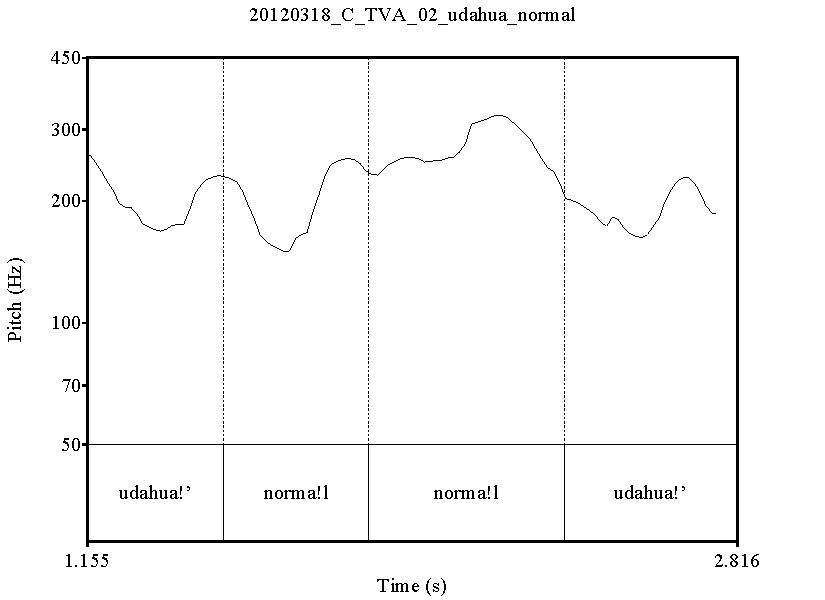
\includegraphics[height=.4\textheight]{gudahuanormal}

The use of the predicate focus construction followed immediately by argument focus may be conceptualized as a discursive structure to its own which exploits the ``parallelism'' \citep{jakobson1966,fox1977} of the mirror image syntactic structures employed.\footnote{I thank Richard Rhodes for useful comments on this point.} One of the functions of this parallelism, or ``chiastic structure'' \citep{silverstein1984}, is to help the speaker extend his speaking turn for an additional intonation unit. At the same time, the predicate focus plus argument focus combination together mark the end of the speaker's turn. The speaker cedes the floor, though not before providing a captivating end to the re-telling of a seemingly routine and uneventful night of eating. More importantly, the use of the chiastic structure binds the two intonation units into a couplet to be interpreted together.

This combined use of predicate focus plus argument focus as a chiastic structure is employed often in conversation between ZAI speakers. Below is a second example. Here, the speaker is talking about his participation in an international marathon in Mexico City 25 years prior and uses the chiastic structure of predicate focus plus argument focus in lines 2-3 to highlight his young age at the time:

\ea (T and M, 19 March 2012, 0:58.0-1:04.0)
\begin{itemize}

\item[01 T:] 
\glll dxi bixoo\~{n}\'{e} jaa marat\'{o}n internacion\'{a}l qu\'{e} l\'{a}, \\
dxi bi-xoo\~{n}e=a'\textsuperscript{H} jaa marat\'{o}!n internacional\textsuperscript{H} que\textsuperscript{LH} la\textsuperscript{H} \\
when \textsc{compl}-run=\textsc{1sg} \textsc{intj} marathon international \textsc{dem} \textsc{la} \\
\glt `When I ran the international marathon,'


\item[02 T:] 
\glll m\'{a} nap\'{a} veintid\'{o}s iza \\
 ma'\textsuperscript{H} n-apa=a'\textsuperscript{H} veintidos\textsuperscript{H} iza \\
already \textsc{hab}-have=\textsc{1sg} twenty-two year \\
\glt `I was twenty-two years old' 


\item[03 T:] 
\glll veintid\'{o}s iza nap\'{a} dxiqu\v{e} \\
veintidos\textsuperscript{H} iza n-apa=a'\textsuperscript{H} dxique\textsuperscript{LH} \\
twenty-two year \textsc{hab}-have=\textsc{1sg} then \\
\glt `I was TWENTY-TWO then' 


\end{itemize}
\z

After beginning his turn with a \textsc{la}-marked adverbial phrase in line 1 which introduces the event of the international marathon as topical, the speaker uses a predicate focus construction in line 2 to remark on his age at the time. In line 3, the speaker repeats the semantically equivalent utterance, this time using an argument focus construction in which his age appears pre-verbally. 


In the final example, also from conversation, a similar use of the parallel, chiastic structure is used. This time the particle \textsc{nga} can be observed. In the first two lines, T asks C what kinds of crops his father used to grow on his plot of land and whether he had cattle. C responds in lines 3-8.

\ea (T and C, 27 Sept 2012, 1:33.5-1:49.0)
\begin{itemize}

\item[01 T:]
\glll {?`}xi b\'{i}dx\'{i}'babe y\'{a}'? \\
xi\textsuperscript{LH} bi-dxi'\textsuperscript{H}ba=be\textsuperscript{LH} ya' \\
what \textsc{compl}-grow=\textsc{3.hum} \textsc{q} \\
\glt `What did he grow?'



\item[02 T:]
\glll {?`}gupabe y\v{u}z\'{e} l\'{a}? \\
gu-apa=be\textsuperscript{LH} yu\textsuperscript{LH}ze\textsuperscript{LH} la\textsuperscript{H} \\
\textsc{compl}-have=\textsc{3.hum} cattle \textsc{q} \\
\glt `Did he have cattle?'


\item[03 C:] 
\glll bidx\'{i}'babe p\v{u}ru xub\'{a}' \\
bi-dxi'\textsuperscript{H}ba=be\textsuperscript{LH} pu\textsuperscript{LH}ru xuba'\textsuperscript{H} \\
\textsc{compl}-grow=\textsc{3.hum} only maize \\
\glt `He only grew maize'  


\item[04 C:] 
\glll purt\'{i} cheri l\'{a},  \\
purti\textsuperscript{H} cheri\textsuperscript{LH} la\textsuperscript{H}  \\
because here \textsc{la} \\
\glt `Because around here,'


\item[05 C:] 
\glll p\v{u}ru ng\v{a} ng\'{a} rudx\'{i}'bacab\v{e} \\
pu\textsuperscript{LH}ru nga\textsuperscript{LH} nga\textsuperscript{H} ru-dxi'\textsuperscript{H}ba=ca=be \\
only \textsc{dem} \textsc{nga} \textsc{hab}-grow=\textsc{pl=3.hum} \\
\glt `Only that is what they grow' 


\item[06 C:]
\glll m\'{a} p\v{u}ru xub\'{a}'  \\
ma'\textsuperscript{H} pu\textsuperscript{LH}ru xuba'\textsuperscript{H}   \\
already only maize \\
\glt `Now just maize'  


\item[07 C:] 
\glll ira \'{i}x\'{e} c\'{a}mpes\v{i}nu nuu l\v{a}d\'{u} r\'{i} l\'{a}, \\
guira'\textsuperscript{LH} ixe\textsuperscript{LH} campesi\textsuperscript{LH}nu n-uu\textsuperscript{LH} la\textsuperscript{LH}du ri'\textsuperscript{H}  la\textsuperscript{H} \\
all all peasant \textsc{stat}-be side \textsc{dem} \textsc{la} \\
\glt 'All the peasants here (lit. 'that are on this side')'


\item[08 C:]
\glll m\'{a} p\v{u}ru xub\'{a} rudx\'{i}'bacab\v{e}  \\        
ma'\textsuperscript{H} pu\textsuperscript{LH}ru xuba'\textsuperscript{H} r.u=dxi'\textsuperscript{H}ba=ca=be \textsuperscript{LH}  \\
now just maize \textsc{hab}=grow=\textsc{pl=3.hum}  \\
\glt `Now they grow only maize' 

\end{itemize}
\z

In response to T's question in lines 1-2, C responds with a predicate focus construction in line 3, saying that his father only cultivated maize. In lines 4- 5, he continues this thought stating that in that region maize is the only crop that was grown and does so using an argument focus construction involving the particle \textsc{nga}. He repeats this thought again in line 6 in a verb-less clause. He ends his turn in lines 7-8 with an argument focus construction that is a mirror image of line 3. 

Again, the use of the predicate focus construction followed immediately by argument focus can be conceptualized as a chiastic structure that exploits the parallelism of the mirror image syntactic structures employed. In using this parallel, chiastic structure, the two intonation units are bound into a couplet to be interpreted together, and the speaker extends his speaking turn for an additional intonation unit, with the second part, the argument focus construction, marking the end of the speaker's turn, thereby ceding the floor.


\section{Summary and conclusions}


In summary, this chapter explored the range of types of focus constructions in the ZAI data. As we saw, in the information structure of ZAI, sentence focus and predicate focus constructions are consistently verb-initial and argument focus constructions contain either pre-verbal constituents (within the clause) or, alternatively, may be verb-initial. A summary of these facts is shown in \tabref{allfocus}:


\begin{table}
\caption{\small{Focus constructions in ZAI}}
\begin{tabular}{l l l  l l}
& & & & \\
 & Context & Example & Focus type & Constituent  \\
& & & & order \\
 
\lsptoprule
a. &  How's your car? & \textit{guxhii\~{n}en\v{i}} & \textsc{Predicate} & \textsc{V-initial} \\
 &   &  & \textsc{focus} &  \\
b. & What happened? & \textit{guxhii\~{n}e xcoch\'{e}'} & \textsc{Sentence} & \textsc{V-initial} \\
 &  &  & \textsc{focus} & \\
c. & I heard your & \textit{xcoch\'{e} guxhii\~{n}e'} & \textsc{Argument} & pre-verbal NP \\
 & motorcycle broke down  &  & \textsc{focus} & \\
 \end{tabular}
\end{table}\label{allfocus}


In addition, this chapter showed that there is no evidence for pitch accents directly associated with focal material. However, elements may display various prosodic properties-- longer duration, higher pitch register, and greater pitch range-- related to their position within a given intonation unit. In particular, focused elements, be they nominal or verbal constituents, tend to occur in prosodically more prominent positions, i.e. beginnings of intonation units. Pre-verbal elements, for their part, are exclusively part of the focus domain. This was viewed as a possible prosodic motivation for the focus domain being associated primarily with the initial position, be it the verb in a verb-initial construction or a pre-verbal element.

These observations led us to examine the place of ZAI within the typology of focus structure proposed by \citet{vanvalin1999}. First, because arguments as well as non-arguments may occur pre- or post-verbally, we described ZAI as syntactically relatively flexible. Second, given that focused constituents can appear either pre-verbally or post-verbally, it was determined that the potential focus domain in ZAI is also relatively flexible. In broad focus constructions (i.e. sentence or predicate focus), the focus domain is post-verbal and, in narrow focus constructions, there is a strong preference for focused constituents to appear pre-verbally (though post-verbal focused constituents are possible). Lexical NPs, whether pre- or post-verbal, are usually part of the focus domain, as are pre-verbal independent pronouns.\footnote{Pre-verbal lexical NPs may also represent topicalized NPs (cf. \sectref{topicalizationsection}).} In contrast, pronominal enclitics are always topical. 

However, it does appear that focus structure is more rigid than syntax, since focus structure can motivate certain syntactic arrangements while the reverse never holds. That is, syntactic structure does not appear to motivate changes in the focus domain. Therefore, ZAI may tend more towards the Italian-type rather than the Russian-type (cf. \tabref{zapfoctyp}). 

Finally, the chapter concluded with a discussion of a conversational strategy used by ZAI speakers involving the successive use of predicate focus and argument focus to accomplish specific conversational goals. The use of the predicate focus construction followed immediately by argument focus was analyzed as a chiastic structure that exploits the parallelism of the mirror image syntactic structures employed. In using this chiastic structure, the two intonation units are bound into a couplet to be interpreted together, and the speaker extends his speaking turn for an additional intonation unit, with the second part, the argument focus construction, marking the end of the speaker's turn, ceding the floor.



